\section{Contrail Detection}
\label{sec:intro}

\subsection{Introduction}

Contrail detection is an essential component towards understanding the impact and mitigation of contrails. Being able to detect contrails with high accuracy is a necessary capability in order to evaluate and compare contrail predictive models, to track contrails through their lifespan and measure the amount of heat that they trap, and ultimately to verify the effectiveness of flight path diversion efforts.

Remote sensing satellites, equipped with state-of-the-art sensors, such as the Advanced Baseline Imager (ABI) on the Geostationary Operational Environmental Satellites (GOES) \cite{goes} have allowed for reliable and consistent environmental observations. Compared to Polar-orbiting Operational Environmental Satellites (POES) such as the Suomi or Sentinel satellites, GOES maintains constant observation over a fixed area with relatively higher temporal resolution but at the cost of lower spatial resolution. With 2 kilometer spatial resolution in the infrared bands, GOES imagery in not sufficient to capture the initial formation of young contrails, but is able to capture the more mature stages of contrails if they continue to spread out. GOES's coarser resolution narrows our focus on the contrails with the largest climate impact since persistent contrails that have expanded sufficiently to be observable at 2 kilometer resolution are associated with more significant warming effects \cite{warm, persist}. Additionally, the proposed contrail predictive model will be at 3 kilometer resolution, thus reducing the utility of higher resolution contrail detection. 

\subsection{Related Work}

In the last 25 years, contrails have primarily been detected in POES imagery using image processing techniques such as the Mannstein et al. algorithm \cite{mannstein} that applies a series of hand engineered convolution and thresholding operations to infrared imagery. More recently, a method for tracking the life cycle of contrails that uses the aforementioned Mannstein et al. algorithm on POES imagery for early stage detection and then uses a tracking algorithm on GOES imagery for later stage contrail evolution \cite{track}. POES satellites are often constrained by a single pass per day over a given area of interest, limiting the ability to support contrail avoidance.

With the introduction of large human-labeled contrail datasets \cite{opencontrails, landsat}, more recent studies have applied deep learning based contrail detection models \cite{opencontrails, covid} with GOES imagery. While deep learning approaches have the potential to better support contrail avoidance predictions, there has not been a direct performance analysis between the Mannstein et al. method and the deep learning models. Quantifying the effectiveness of contrail detection methods is crucial for accurate assessment of the cost and benefits of contrail predictive models. False positives of a high probability area for contrail formation would increase costs of fuel consumption for flights to take unnecessary avoidance measures. False negatives, where a flight creates preventable contrail formations, would decrease the utility of implementing contrail predictive models. 


\begin{figure}
\centering

\begin{subfigure}[t]{.49\linewidth}
  \centering
    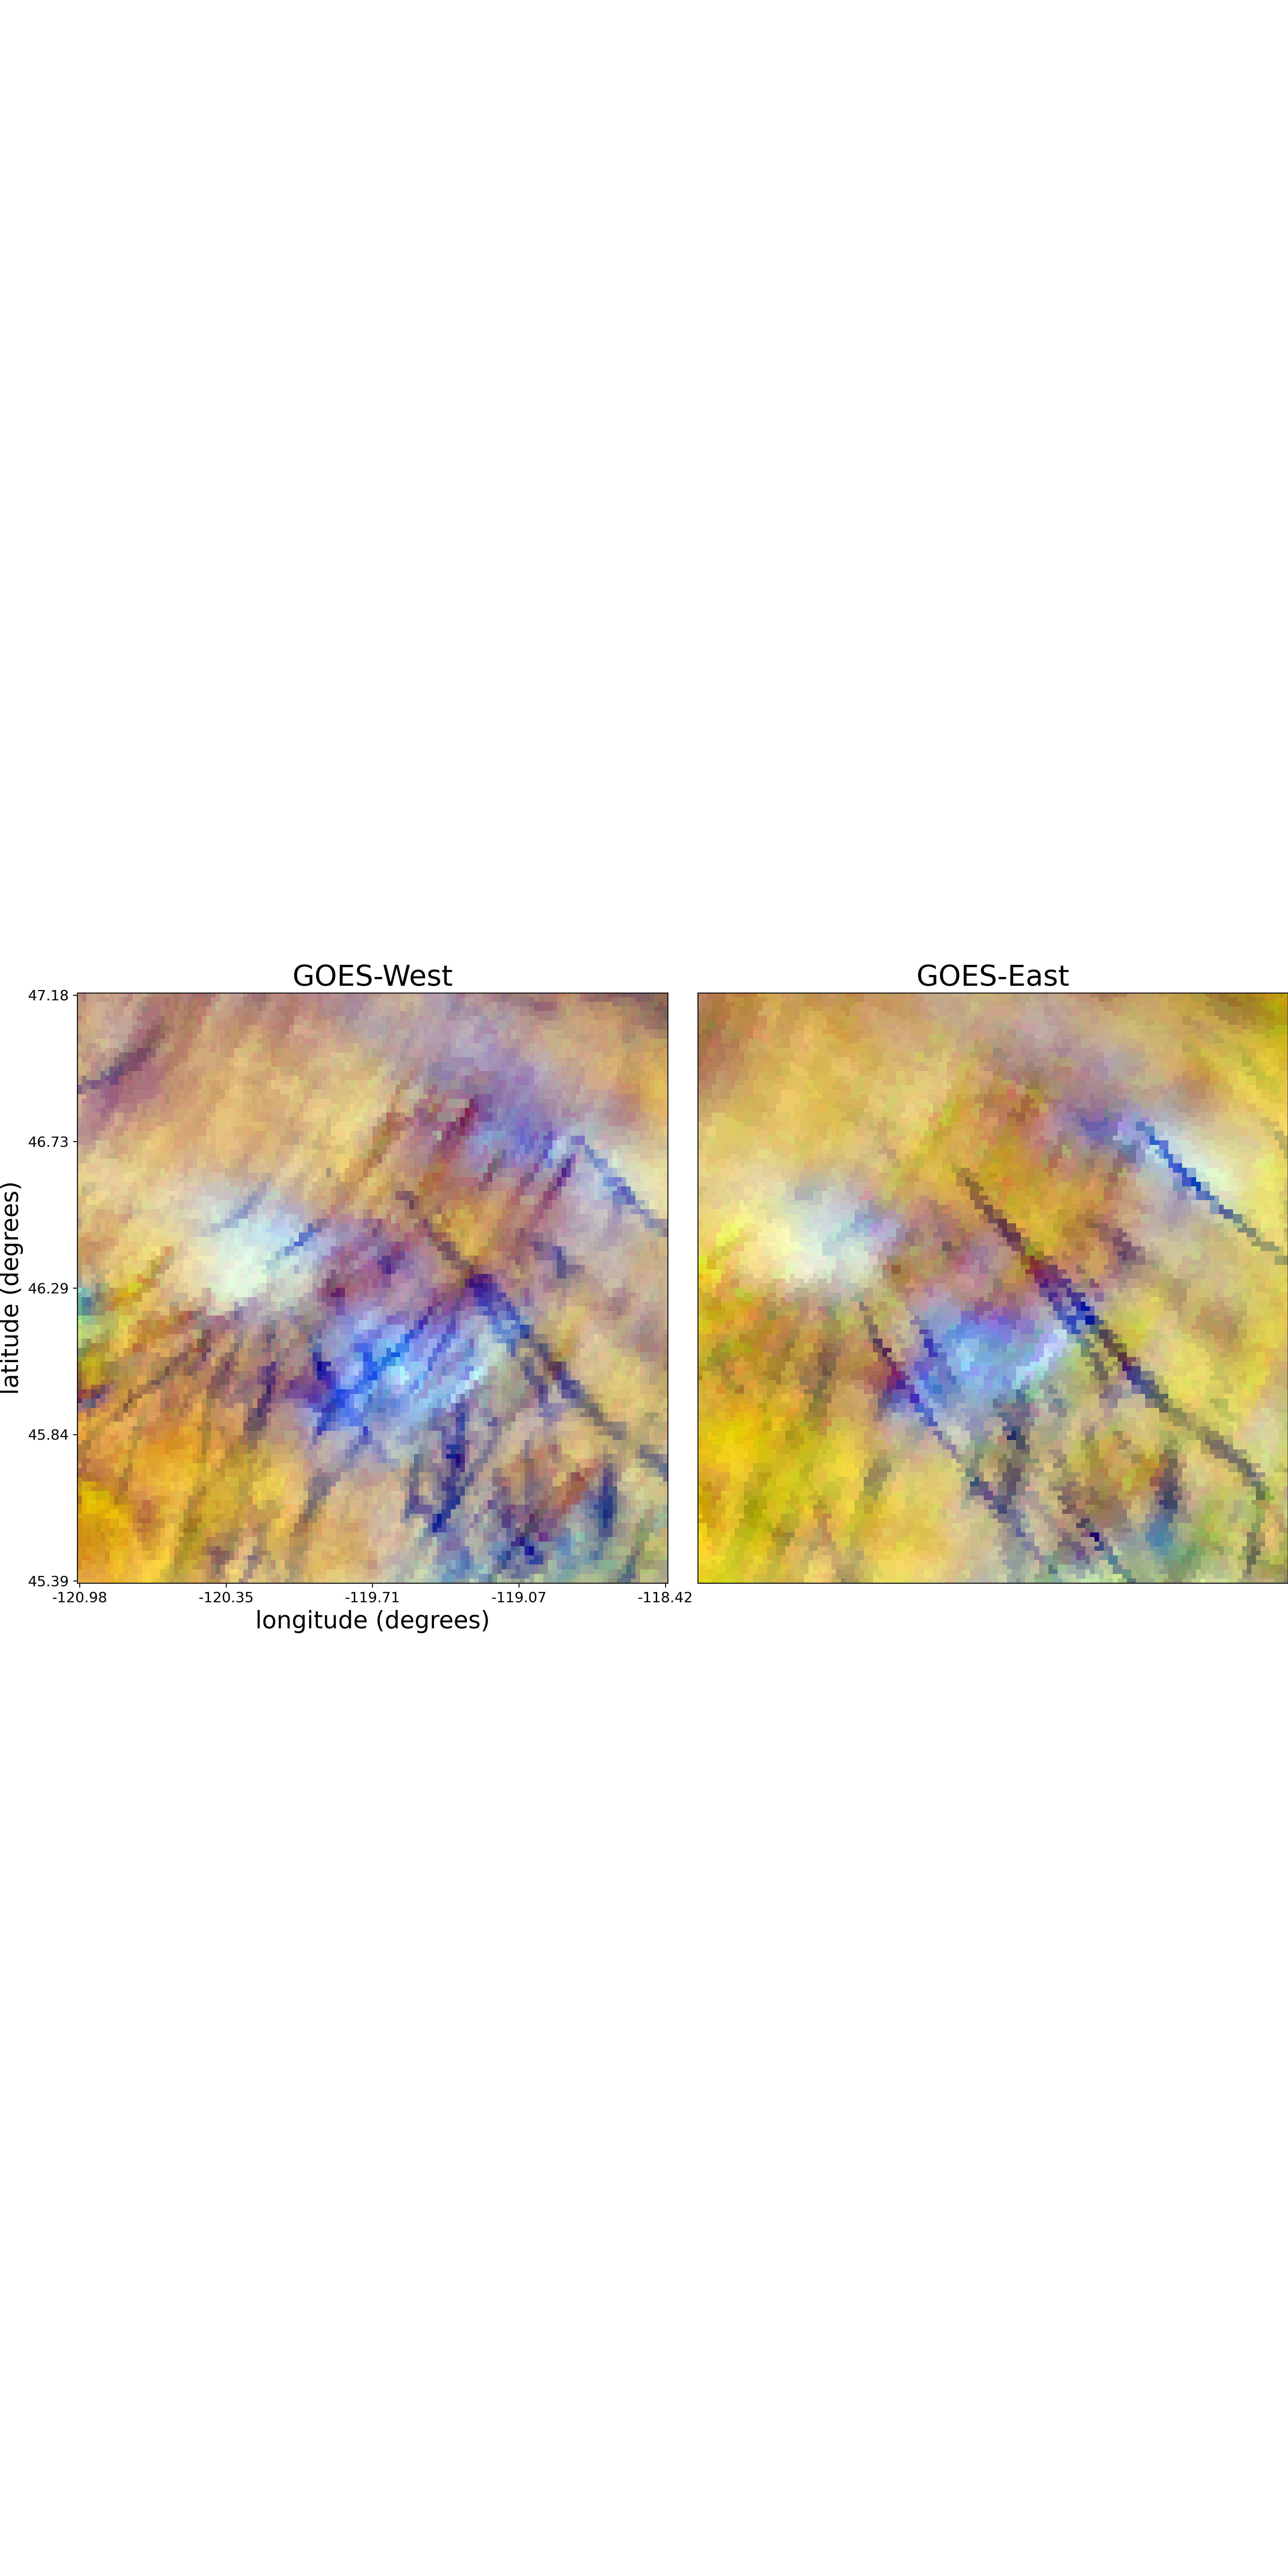
\includegraphics[width=\linewidth]{figures/west_best.png}
    \caption{GOES imagery from 2025/03/11 15:50 UTC.}
  \label{best_west}
\end{subfigure}
\hspace{.01cm}
\begin{subfigure}[t]{.49\linewidth}
  \centering
    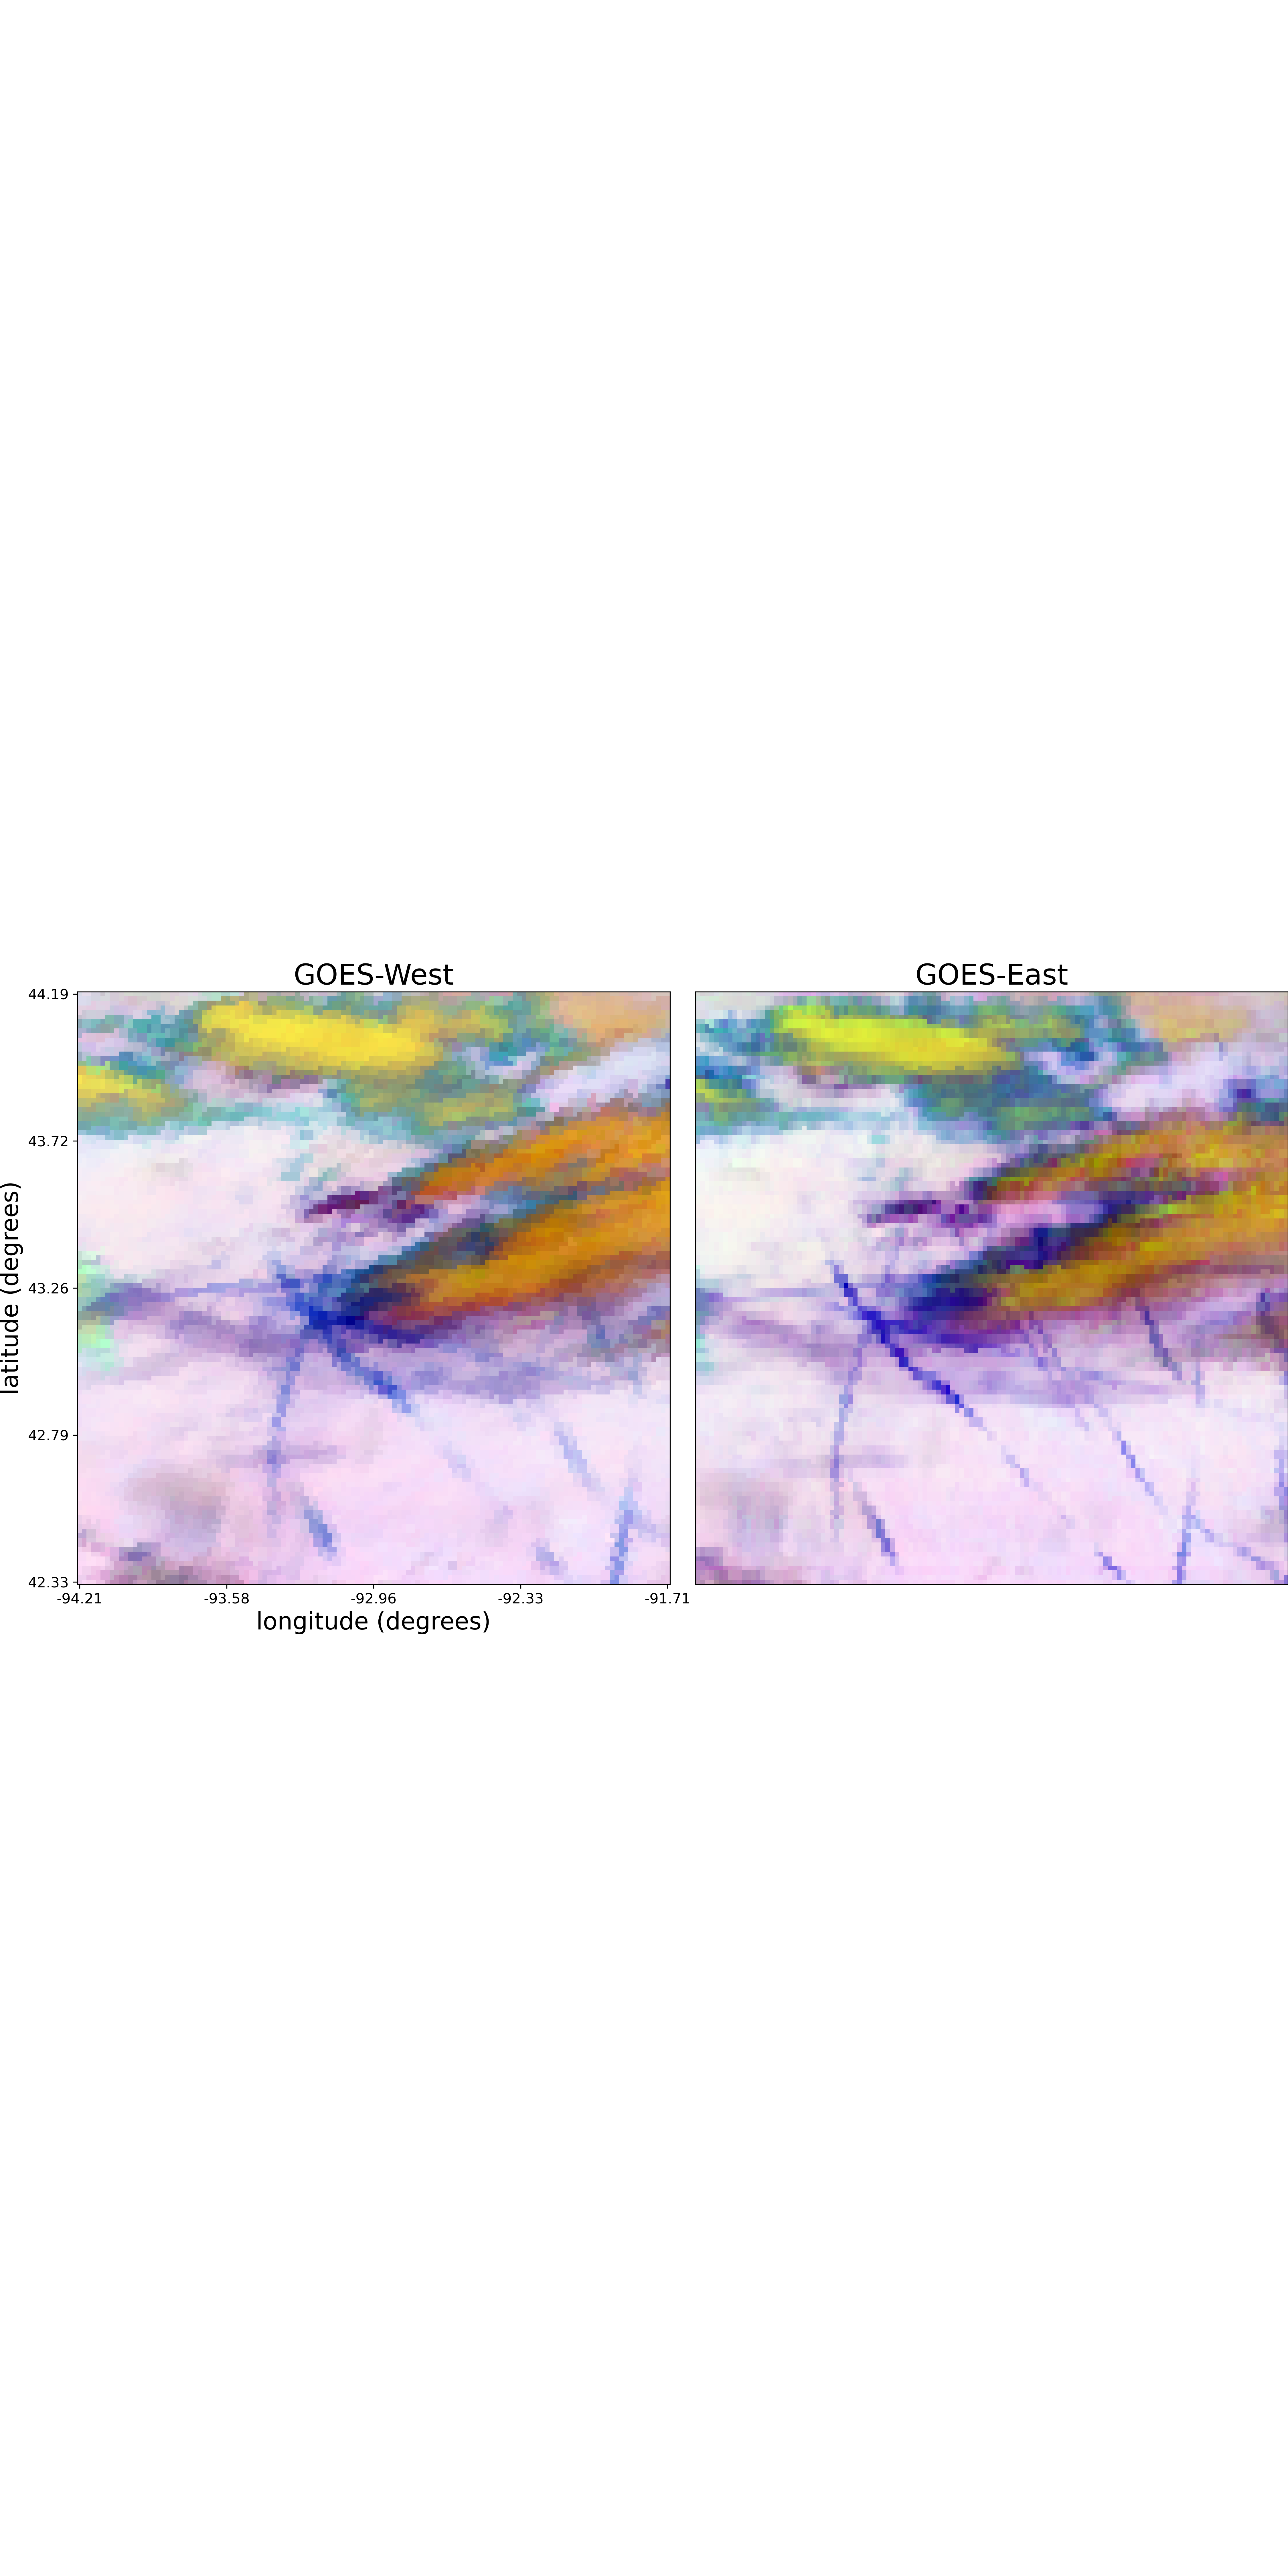
\includegraphics[width=\textwidth]{figures/east_best.png}
    \caption{GOES imagery from 2025/02/28 13:30 UTC.}
  \label{best_east}
\end{subfigure}

\begin{subfigure}[t]{.49\linewidth}
  \centering
    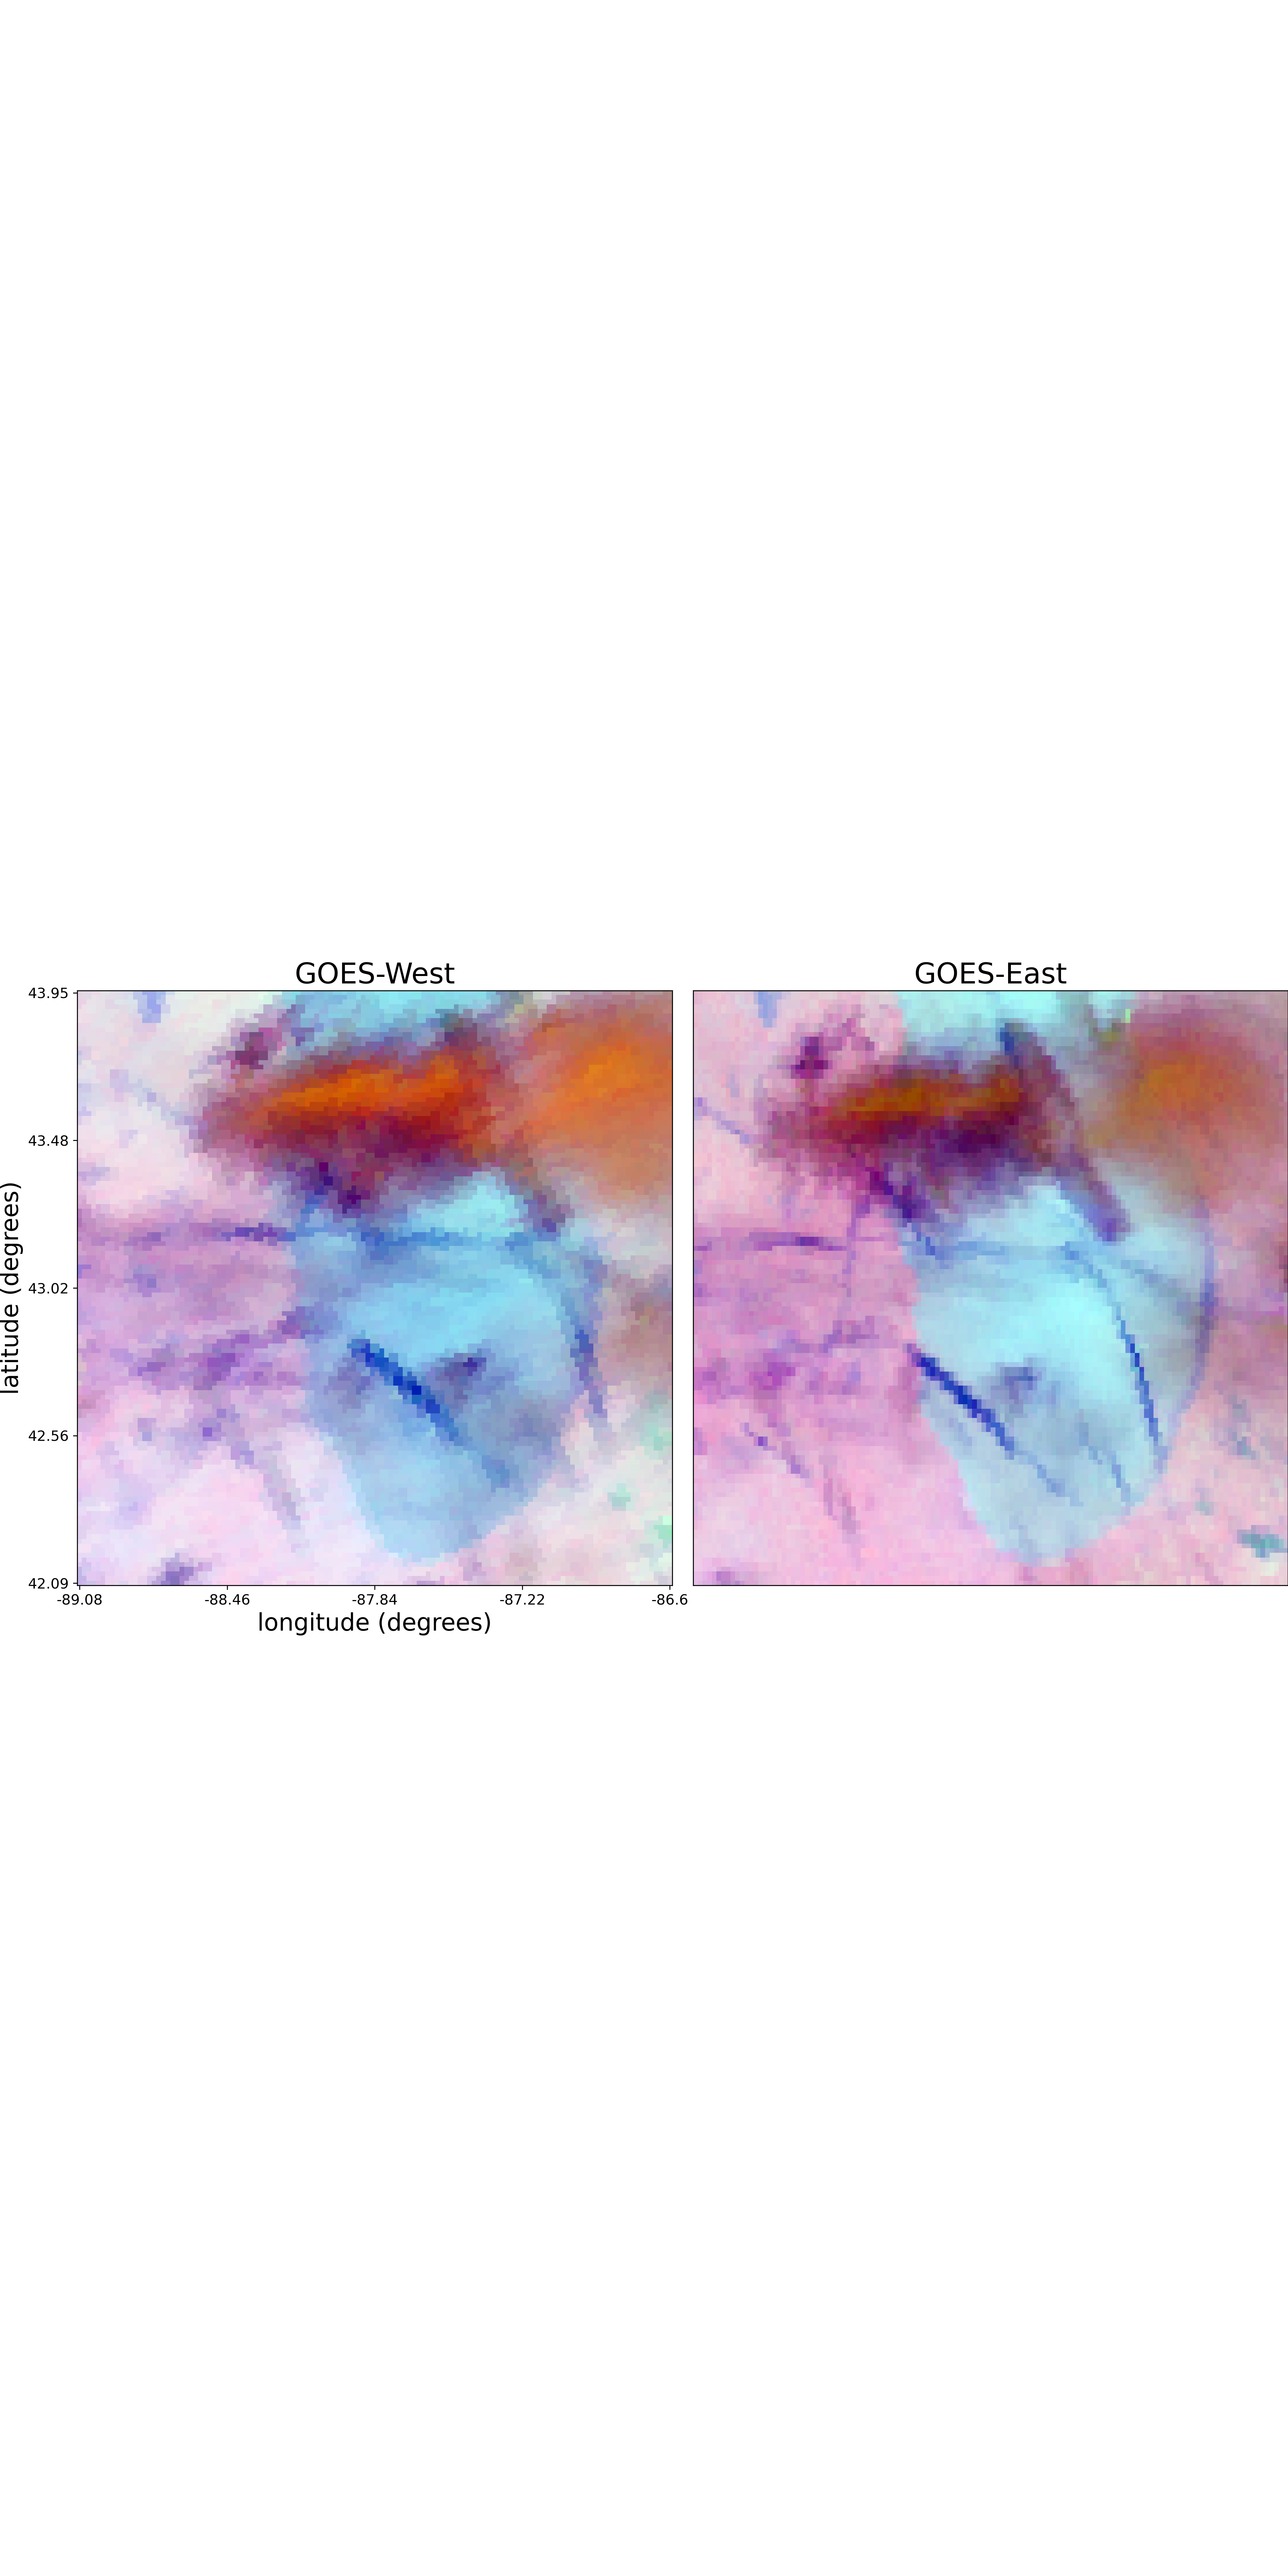
\includegraphics[width=\textwidth]{figures/superior_parallax.png}
    \caption{GOES imagery from 2025/02/28 05:40 UTC with contrails over Lake Michigan to visualize the parallax difference between GOES-West and GOES-East.}
  \label{parallax1}
\end{subfigure}
\hspace{.01cm}
\begin{subfigure}[t]{.49\linewidth}
  \centering
    \includegraphics[width=\textwidth]{figures/superior_parallax_2.png}
    \caption{Same as figure \ref{parallax1} but with contrail labels from GOES-West (black) and GOES-East (white) with the parallax distance in red corresponding to a difference of 16 pixels or 32 km.}
  \label{parallax2}
\end{subfigure}

\caption{Side-by-side comparisons of ash composites for GOES-West and GOES-East imagery using bands 11, 13, 14 and 15 (8.4\(\mu\)m, 10.3\(\mu\)m, 11.2\(\mu\)m and 12.3\(\mu\)m) to show cirrus as dark blue.}
\label{goes_img}
\end{figure}

\subsection{Proposed Work}

\subsubsection{GOES-East Deep Learning Detection Model}
While the OpenContrail project has made their human-labeled dataset publicly available, the benchmark models presented in the paper \cite{opencontrails} are not made public. The architecture used for the \cite{opencontrails} baseline models are ResNet \cite{resnet} and DeepLabV3+ \cite{deeplab} and are no longer considered state-of-the-art within semantic segmentation. We propose to use SegFormer \cite{segformer} that uses state-of-the-art attention mechanisms optimized for computational efficiency especially for multi-resolution objects such as contrails. To train the deep learning model we will use the OpenContrail dataset that is composed of 16 bands of GOES-East imagery for training data and human-labeled contrails for training labels. The input data to the trained model will be GOES-East imagery for a specified time window and the output of the model will be a geospatial vector file with the geometry of detected contrails within that time window.

\subsubsection{Analysis of Mannstein et al. Algorithm}

The OpenContrail dataset \cite{opencontrails} presents a series of deep learning models for a benchmark while the Landsat-8 contrail dataset \cite{landsat} uses the Mannstein et al. algorithm to show their baseline results. Given the importance of model and dataset accuracy, instead of using one type of baseline model, we propose to use both the Mannstein et al. algorithm along with our trained GOES-East deep learning model to quantify the quality of the dataset. Along with providing insights on the reliability of the dataset, this comparison will support whether a deep learning model offers better detection capabilities than the Mannstein et al. algorithm on the OpenContrail test set. Despite the algorithm being developed for the difference between the 12\(\mu\)m and 10.8\(\mu\)m bands on the AVHRR instrument \cite{mannstein}, it has tunable parameters for adaptation to new instruments. We will perform parameter tuning to get the algorithm compatible with bands 15 (12.3\(\mu\)m) and 13 (10.3\(\mu\)m) available on the GOES-ABI.

\subsubsection{GOES-West Derived Dataset and Model}
The OpenContrail model solely utilizes GOES-East imagery, but GOES-West can provide higher quality observations of the West coast (figure \ref{best_west}) with a corresponding relationship for GOES-East on the East coast (figure \ref{best_east}). Preliminary figures, \ref{best_west} and \ref{best_east}, demonstrate how contrails can be observable in one satellite but not the other. Since OpenContrail dataset only provides annotations associated with GOES-East, it may be missing contrails that are only visible by GOES-West. Due to the parallax effect (figure \ref{parallax1}-\ref{parallax2}) between GOES-East and West for high altitude clouds such as contrails, it is not possible to immediately match up the contrail labels to the GOES-West imagery. We will need to solve for the shift in observed location in order to build the GOES-West dataset. From that newly introduced dataset, we will then train a model that will detect contrails in GOES-West imagery. This will allow us to compare the GOES-West model to the GOES-East model and provide a tool for analysis on parallax shift and its relationship to contrail altitude.

\subsubsection{Contrail Altitude Approximation from Satellite Observation}
Matching a contrail detection to its corresponding flight altitude is critical information needed to validate a contrail predictive model. In high flight traffic areas, it can be difficult to match a contrail to its correct flight altitude data. Furthermore, even when accurately matched, it can be computationally intensive to find the data that is often on a delayed release \cite{flight}. Optimal functionality would be to be able to determine contrail altitude directly from satellite imagery. Contrail altitude estimation using GOES-East has been shown effective \cite{alt}, but does not use the parallax information available from using both GOES-East and West in conjunction. We show in figure \ref{parallax2} that if we are able to match the GOES-West contrail detection to the corresponding GOES-East detection, we will be able to determine the parallax distance in order to calculate the contrail altitude.

\subsubsection{Study Contrails with Highest Impacts}
While the primary focus of this work is to predict and mitigate persistent contrails observable by GOES's 2km resolution, we are also interested in understanding the atmospheric conditions required for persistent contrails to continue evolving into lasting fields of cirrus clouds. When contrails form cirrus fields, the radiative impact is larger than the typical persistent contrail. We propose to use a cloud regime classification model currently in development to match contrail detections to down-the-line areas of cirrus clouds.

